% compile with XeLaTeX
% this template was created by salim bou 
\documentclass[dvipsnames,mathserif]{beamer}
\mode<presentation>
\usepackage{tikz}
\usepackage{pgfplots}
\pgfplotsset{compat=1.18}
\usetikzlibrary{calc}
\usepackage{listings}
\usepackage{xcolor}
\usepackage[table]{xcolor}
\usepackage{multicol}
\usepackage{multirow}
\usepackage{arabtex}
\usepackage{mathtools}
 \usepackage[LAE,T1]{fontenc}
%\usepackage[arabic,french,english]{babel}
\usepackage{tabularx}
\usepackage{hyperref}
\usepackage{polyglossia}
\setdefaultlanguage[numerals=maghrib,locale=algeria]{arabic} % locale=mashriq, libya, algeria, tunisia, morocco, or mauritania  for names of months in \date 
%\setotherlanguage{english}
\newfontfamily\arabicfont[Script=Arabic]{Amiri}
\newfontfamily\arabicfontsf[Script=Arabic]{Amiri}

\usetikzlibrary{arrows,shapes,backgrounds}

 \newcommand{\rtx}[1]{\textcolor{red}{#1}}
 
\newcommand{\fr}{\selectlanguage{french}}

\newcommand{\bltx}[1]{\textcolor{blue}{#1}}
\newcommand{\grtx}[1]{\textcolor{green}{#1}}
\newcommand{\blcommand}[2]{\bltx{\bf$\backslash$#1}\{\bf #2\}}
\newcommand{\grcommand}[1]{\grtx{\bf #1}}
%--------------------------------------------------------------
\newcommand{\sncommand}[1]{\bltx{\bf#1$\backslash$}}
\newcommand{\dbcommand}[2]{\{\bf #2\}\bltx{\bf#1$\backslash$}}

\newcommand{\opcommand}[3]{\{\bf #3\}[\grtx{\bf #2}]\bltx{\bf#1$\backslash$}}
\newcommand{\opcommandtwo}[3]{\{\bf #3\}[#2]\bltx{\bf#1$\backslash$}}
%------------------------------------------------------------
\newenvironment{mycode}
    {%\RTListe
    \begin{center}
    \begin{tabular}{|p{0.9\textwidth}|}
    \hline
    \begin{flushright}
    }
    {
    \end{flushright}
    \\\hline
    \end{tabular} 
    \end{center}
    }
 
\newcommand{\gfcb}[1]{%
    \fcolorbox{white}{gray!10!}{\quad\strut #1\quad}
    } % gfcb := gray fcolorbox
\newcommand{\cop}[1]{%
    \ensuremath{\quad\longrightarrow\quad #1}
    \gfcb{\texttt{\detokenize{#1}}} 
    %\ensuremath{\quad\longrightarrow\quad #1}
    } % cop := code output



%\usetheme{Madrid}
\usetheme{modprogressbarMAHER}
%\usecolortheme{crane}
\usetikzlibrary{fadings, backgrounds}
\tikzfading[name=fade out, inner color=transparent!100, outer color=transparent!40]
\tikzfading[name=fade in, inner color=transparent!100, outer color=transparent!0]
%\usetikzlibrary{mindmap}
\usetikzlibrary{shadows}
\usetikzlibrary{shapes,arrows,positioning,automata,backgrounds,calc,er,patterns}

%\usepackage{tikz-feynman}

\tikzfeynmanset{compat=1.0.0}
\usetikzlibrary{decorations.pathmorphing, patterns,shapes}

\usepackage[beamer]{hf-tikz}
 
\usetikzlibrary{overlay-beamer-styles}
\tikzset{
	highlight on/.style={alt={#1{fill=red!80!black,color=red!80!black}{fill=gray!30!white,color=gray!30!white}}},
}

%\tikzset{
%	basic/.style  = {draw, text width=2cm, drop shadow, font=\sffamily, rectangle},
%	root/.style   = {basic, thin, align=center,
%		fill=gray!45},
%	level 2/.style = {basic, thin,align=center, fill=gray!30,
%		text width=8em},
%	level 3/.style = {basic, thin, align=left, fill=gray!20, text width=6.5em}
%}
 \tikzset{
 	basic/.style  = {draw, text width=4cm, drop shadow, font=\sffamily, rectangle},
 	root/.style   = {basic, rounded corners=2pt, thin, align=center,
 		fill=green!30},
 	level 2/.style = {basic, rounded corners=3pt, thin,align=center, fill=green!60,
 		text width=10em},
 	level 3/.style = {basic, thin, align=left, fill=pink!60, text width=7.8em}
 }
 
\tikzset{
	pivot/.style={
		draw, 
		regular polygon, 
		regular polygon sides = 3, 
		fill = red, 
		node distance = 1cm, 
		minimum height = 2em,
		at = {(0,0)}
	}
}
% for RTL liste
\makeatletter
\newcommand{\RTListe}{\raggedleft\rightskip\leftm}
\newcommand{\leftm}{\@totalleftmargin}
\makeatother



% RTL frame title
\setbeamertemplate{frametitle}
{\vspace*{-1mm}
  \nointerlineskip
    \begin{beamercolorbox}[sep=0.3cm,ht=2.2em,wd=\paperwidth]{frametitle}
        \vbox{}\vskip-2ex%
        \strut\hskip1ex\insertframetitle\strut
        \vskip-0.8ex%
    \end{beamercolorbox}
}


% align subsection in toc
\makeatletter
\setbeamertemplate{subsection in toc}
{\leavevmode\rightskip=5ex%
  \llap{\raise0.1ex\beamer@usesphere{subsection number projected}{bigsphere}\kern1ex}%
  \inserttocsubsection\par%
}
\makeatother

% RTL triangle for itemize
\setbeamertemplate{itemize item}{\scriptsize\raise1.25pt\hbox{\donotcoloroutermaths$\blacktriangleleft$}} 

%\setbeamertemplate{itemize item}{\rule{4pt}{4pt}}

\defbeamertemplate{enumerate item}{square2}
{\LR{
    %
    \hbox{%
    \usebeamerfont*{item projected}%
    \usebeamercolor[bg]{item projected}%
    \vrule width2.25ex height1.85ex depth.4ex%
    \hskip-2.25ex%
    \hbox to2.25ex{%
      \hfil%
      {\color{fg}\insertenumlabel}%
      \hfil}%
  }%
}}

\setbeamertemplate{enumerate item}[square2]

\setbeamertemplate{navigation symbols}{}

%%%%%%%%%%%%%%%%%%%%%%%%%%%%[ blocks ]%%%%%%%%%%%%%%%%%%%%%%%%%%%%%%%%%%%%
\newenvironment<>{problock}[1]{%
	\begin{actionenv}#2%
		\def\insertblocktitle{#1}%
		\par%
		\mode<presentation>{%
			%\setbeamercolor{block title}{fg=white,bg=blue!48!black}
			\setbeamercolor{block body}{fg=white,bg=pbblue}
			%  \setbeamercolor{itemize item}{fg=orange!20!black}
			%  \setbeamertemplate{itemize item}[triangle]
		}%
		\usebeamertemplate{block begin}}
	{\par\usebeamertemplate{block end}\end{actionenv}}
 
%=========================================================================
\begin{document}
\title{كورس مكثف لتعلم الLaTeX على محرر Overleaf}
\logo{
\includegraphics[width=0.5cm]{figs/sudan_logo.png}}
\author[محمد ماهر عبد الرحيم محمد]{         \href{https://www.facebook.com/mohammedmaher8932/}{\it{محمد ماهر عبد الرحيم محمد}}  }
\institute{
    \href{https://www.facebook.com/groups/651884204836245}{\Large{ملتقى الفيزيائيين السودانيين}} 
}
\vspace{-1.cm}
%\date{\today}
%\affil{\it{The Insider Researcher Group, Khartoum, Sudan}\\

\date{18/02/2023}
%---------------------------------------------------------------------------
%---------------------------------------------------------------------------
\begin{frame}
\maketitle
    \begin{center}
        
        
\includegraphics[scale=0.1]{figs/sfp.jpg}
        
\includegraphics[scale=0.2]{figs/online-editor-2.png}
        
\includegraphics[scale=0.1]{figs/sfp.jpg}
    \end{center}

\end{frame}
%---------------------------------------------------------------------------
%---------------------------------------------------------------------------

%==========================================================
%////////////////////////////////////////////////////////////////////////////////////
%===================================================================================
\begin{frame}[plain]
    \addtocounter{framenumber}{-1}
    \begin{problock}{}
        \LARGE
        \vfill
        \centerline{\bf \textcolor{black}{\bf اليوم الثاني: تنسيق \LaTeX{} المتقدم}}
        \vfill
    \end{problock}
\end{frame}
%==========================================================
%==========================================================
\begin{frame}{المحتويات}
    \tableofcontents
\end{frame}
%=========================================================
%=========================================================
\section{إنشاء الجداول على ال\LaTeX }
\begin{frame}{إنشاء الجداول على ال\LaTeX }
\scriptsize
 \vspace{-0.2cm}

     \begin{flushleft}
   \{  مواصفات الأعمدة \} [ الموضع ]  \dbcommand{begin}{ tabular }\\
   محتوى الجدول
   \\
    \dbcommand{end}{ tabular }\\
    \end{flushleft}
 
\centering
     \begin{tabular}{|c|c|}
     \hline
        مواصفات الأعمدة  & الغرض \\
        \hline\hline
        l  & عمود متموضع ناحية لليسار\\
        \hline
        c  & عمود متموضغ في المنتصف\\
        \hline
        r  & عمود متموضع ناحية اليمين \\
        \hline
        \{ 'width' \} p & عمود فقرة مع محاذاة النص عموديًا في الأعلى \\
        \hline
        \{ 'width' \} m &  عمود فقرة مع محاذاة النص عموديًا في المنتصف\\
        \hline
       \{ 'width' \} b & عمود فقرة مع محاذاة النص عموديًا في الاسفل\\
        \hline
        | & خط رأسي\\
        \hline
        || &  خطان رأسيان\\
        \hline
     \end{tabular}
\end{frame}
%=========================================================
\begin{frame}{موضع الجدول و اجزاء محتويات الجدول}
 \begin{flushleft}
   \{  مواصفات الأعمدة \} [ الموضع ]  \dbcommand{begin}{ tabular }\\
   محتوى الجدول
   \\
    \dbcommand{end}{ tabular }\\
    \end{flushleft}
\begin{center}
\begin{tabular}{|c|c|}
    \hline
    t  &  أعلى الصفحة\\
    \hline
    c  &   منتصف الصفحة\\
    \hline
    b  &  اسفل الصفحة \\
    \hline
\end{tabular}
\end{center}
\centering
 \begin{tabular}{|c|c|}
 \hline
     \&  & الفاصلة بين الأعمدة \\
    \hline 
    $\backslash\backslash$  & بداية صف جديد\\
    \hline
    hline$\backslash$  & خط أفقي\\
    \hline
    newline$\backslash$   & سطر جديد \\
    \hline
    cline(i-j)$\backslash$ & خط أفقي جزئي يبدأ في العمود i وينتهي في العمود j \\
    \hline
 \end{tabular}
\end{frame}
%=========================================================
\begin{frame}{جدول بسيط}

    \begin{mycode}
     \begin{flushleft}
     \{ c|c \}\dbcommand{begin}{ tabular }\\
   $\backslash\backslash$ \text{B \& A} \\
   \text {D \& C}\\
    \dbcommand{end}{ tabular }\\
    \hrule{\linewidth}\\
     \end{flushleft}
      \begin{table}
    \begin{tabular}{c|c}
        B & A \\
        D &  C
    \end{tabular}
    \end{table}
     \end{mycode}

\end{frame}
%=========================================================
\begin{frame}{وضع الخطوط الفاصلة}
\scriptsize
    \begin{mycode}
     \begin{flushleft}
     \{ c|c \}\dbcommand{begin}{ tabular }\\
     \text{hline$\backslash$}\\
   $\backslash\backslash$ \text{B \& A}\\
    \text{hline$\backslash$}\\
   $\backslash\backslash$ \text {D \& C}\\
    \text{hline$\backslash$}\\
    \dbcommand{end}{ tabular }\\
    \hrule{\linewidth}\\
    \end{flushleft}
    \begin{table}
    \begin{tabular}{c|c}
    \hline
        B & A \\
        \hline
        D &  C\\
    \hline
    \end{tabular}
    \end{table}
     \end{mycode}
\end{frame}
%=========================================================
\begin{frame}{التحكم في اتساع الاعمدة}
\scriptsize
يتطلب وجود الحزمة tablularx:\\
\dbcommand{usepackage}{ tabularx }
    \begin{mycode}
     \begin{flushleft}
    \{ | \{ 2cm \} m | \{ 2cm \} m | \}\dbcommand{begin}{ tabular }\\
     \text{hline$\backslash$}\\
  $\backslash\backslash$  \text{Ahmed \& Huda}\\
    \text{hline$\backslash$}\\
 $\backslash\backslash$   \text {Omar \& Mona}\\
    \text{hline$\backslash$}\\
    \dbcommand{end}{ tabular }\\
    \hrule{\linewidth}\\
      \end{flushleft}
        \begin{table}
    \begin{tabular}{| m{2cm}| m{2cm} |}
    \hline
        Ahmed & Huda \\
        \hline
        Omer &  Mona\\
    \hline
    \end{tabular}
  \end{table}
     \end{mycode}
\end{frame}
%=========================================================
\begin{frame}{دمج الأعمدة}
\scriptsize
\begin{center}
   \{المحتوى\}\{طريقة التنسيق\}     \dbcommand{multicolumn}{عدد الأعمدة}
   
\end{center}

 \begin{mycode}
     \begin{flushleft}
     \{ |c| c|c |\}\dbcommand{begin}{ tabular }\\
     \text{hline$\backslash$}\\
   $\backslash\backslash$ \text{C \& B \& A}\\
    \text{hline$\backslash$}\\
   $\backslash\backslash$ \text{multicolumn\{3\}\{|c|\}\{A+B+C\}$\backslash$}\\
    \text{hline$\backslash$}\\
 $\backslash\backslash$ \text{multicolumn\{2\}\{|l|\}\{B+C\}$\backslash$ \& A}\\
  \text{hline$\backslash$}\\
    \dbcommand{end}{ tabular }\\
      \hrule{\linewidth}\\
     \end{flushleft}
     \begin{table}
    \begin{tabular}{ |c|c|c|}
    \hline
       C & B & A \\
        \hline
        \multicolumn{3}{|c|}{A+B+C}\\
        \hline
        \multicolumn{2}{|l|}{B+C} & A\\
    \hline
    \end{tabular}
        \end{table}
     \newline
   
     \end{mycode}
\end{frame}
%=========================================================
\begin{frame}{دمج الصفوف}
\scriptsize
\begin{center}
   \{المحتوى\}\{  الاتساع\}     \dbcommand{multirow}{عدد الصفوف}
   
\end{center}

 \begin{mycode}
     \begin{flushleft}
     \{ |c| c|c |\}\dbcommand{begin}{ tabular }\\
     \text{hline$\backslash$}\\
   $\backslash\backslash$ \text{C \& B \& A}\\
   $\backslash\backslash$ \text{ C \& B \{ Merge Row \} multirow\{2\}\{*\}$\backslash$}\\
    $\backslash\backslash$ \text{C \& B \& }\\
  \text{hline$\backslash$}\\
    \dbcommand{end}{ tabular }\\
      \hrule{\linewidth}\\
     \end{flushleft}
     \begin{table}
    \begin{tabular}{ |c|c|c|}
    \hline
        C & B & A \\
        \hline
        C & B & \multirow{2}{*}{Row merge}\\
        C & B & \\
    \hline
    \end{tabular}
        \end{table}
     \newline
   
     \end{mycode}
    %\begin{center}
     %   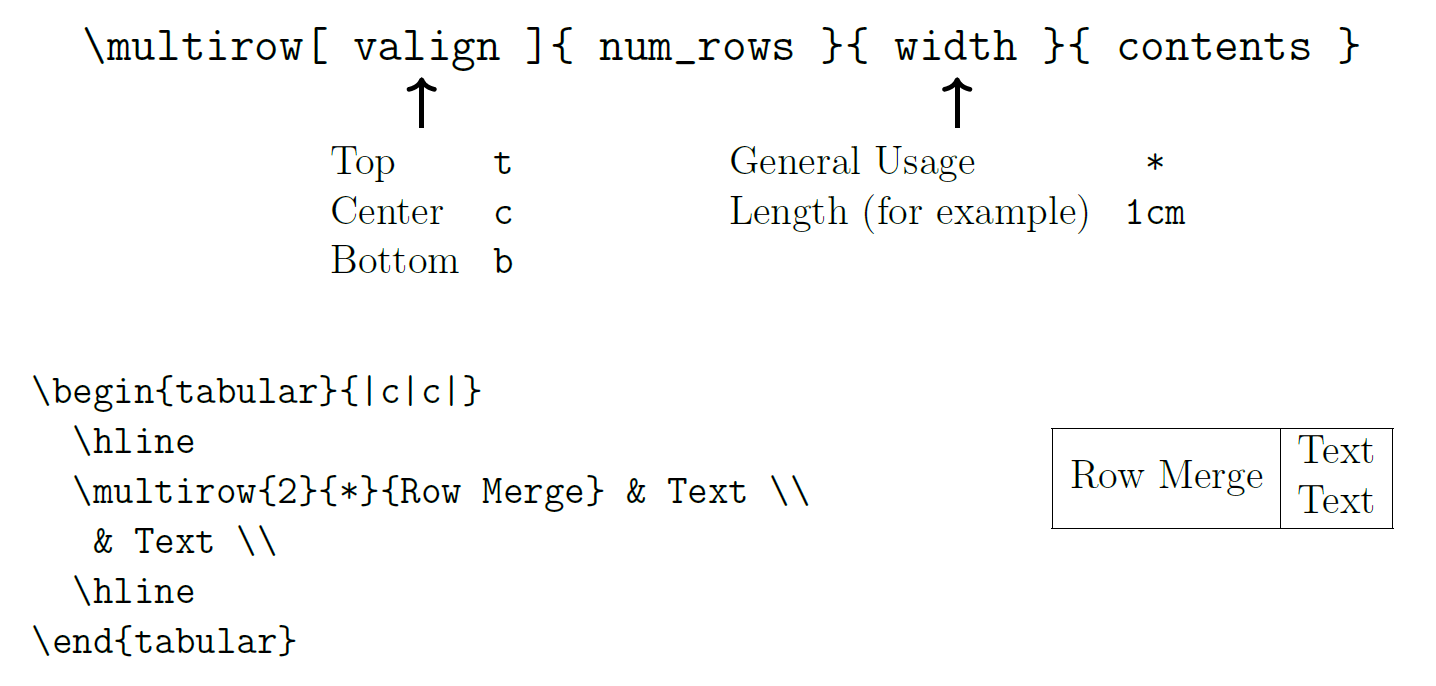
\includegraphics[scale=0.3]{figs/img-4-7.png}
    %\end{center}
\end{frame}
%=========================================================
\begin{frame}{تلوين الجداول}
\scriptsize
    \begin{center}
        \opcommand{usepackage}{ table} { xcolor }
    \end{center}
    
 \begin{mycode}
     \begin{flushleft}
     \{ |c|c| \}\dbcommand{begin}{ tabular }\\
   $\backslash\backslash$ \text{B cellcolor\{purple!30\}$\backslash$\& A cellcolor\{pink!60\}$\backslash$} \\
   \text{hline$\backslash$}\\
   $\backslash\backslash$ \text {D cellcolor\{orange50\}$\backslash$\& C cellcolor\{red!40\}$\backslash$}\\
    \text{hline$\backslash$}\\
    \dbcommand{end}{ tabular }\\
    \end{flushleft}
     \end{mycode}
\vspace{-0.35cm}
 \begin{center}
     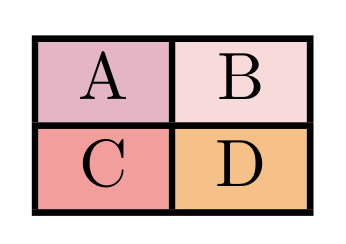
\includegraphics[scale=0.5]{figs/Screenshot-2021-06-01-at-20.29.40.png}
 \end{center}
 \vspace{-0.2cm}
 \begin{center}
        \{لون الصفوف الزوجبية\}\{  لون الصفوف الفردية\}     \dbcommand{rowcolors}{بداية الصف}\\
        \dbcommand{cellcolor}{ لون الخلية}
 \end{center}
\end{frame}
%=========================================================

%=========================================================
\section{تنسيق رياضي متقدم}
\begin{frame}{تنسيق رياضي متقدم}
\scriptsize
\begin{center}
\scriptsize
   \begin{tabular}{|c|c|c|c|}
    \hline
   النوع & صيغ وسط النص & صيغ العرض & الترقيم التلقائي\\ 
    \hline\hline
   البيئة & math & displaymath & equation\\
    \hline
    اختصار ال\LaTeX& (\textbackslash{}...)\textbackslash{}
 & [\textbackslash{}...]\textbackslash{} &\\
    \hline
   أختصار ال\TeX & \$..\$ & \$\$...\$\$ &\\
    \hline
   تعليق &  &  & quation* تمنع الترقيم ، ولكن يتطلب amsmath\\
    \hline
 \end{tabular}  
\end{center}

\begin{center}
  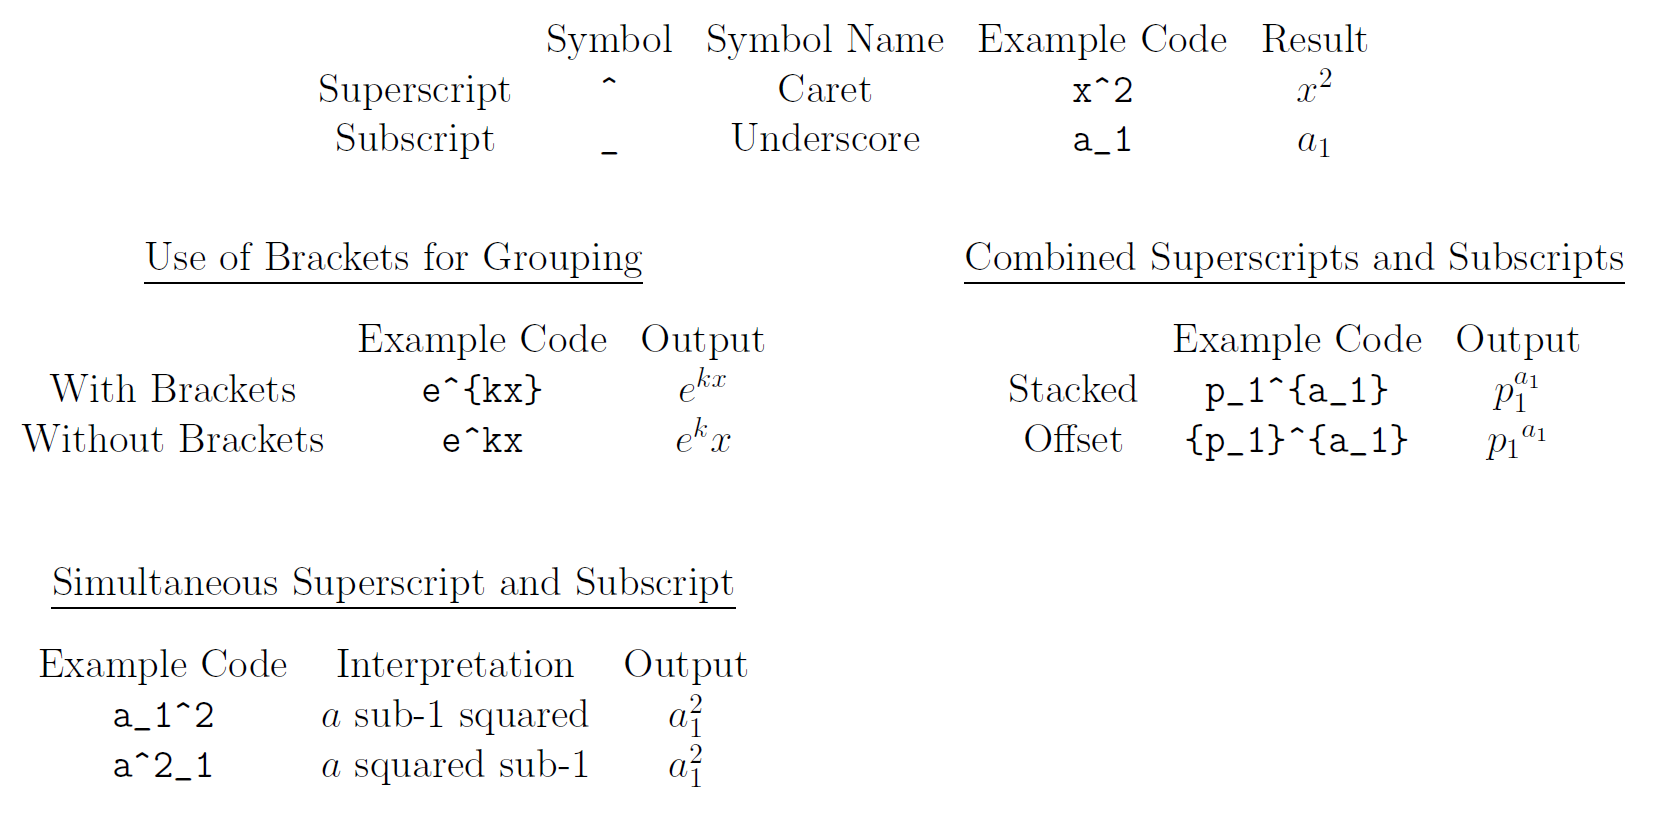
\includegraphics[scale=0.2]{figs/img-3-4.png}
\end{center}
\end{frame}
%=========================================================
\begin{frame}
\begin{center}
    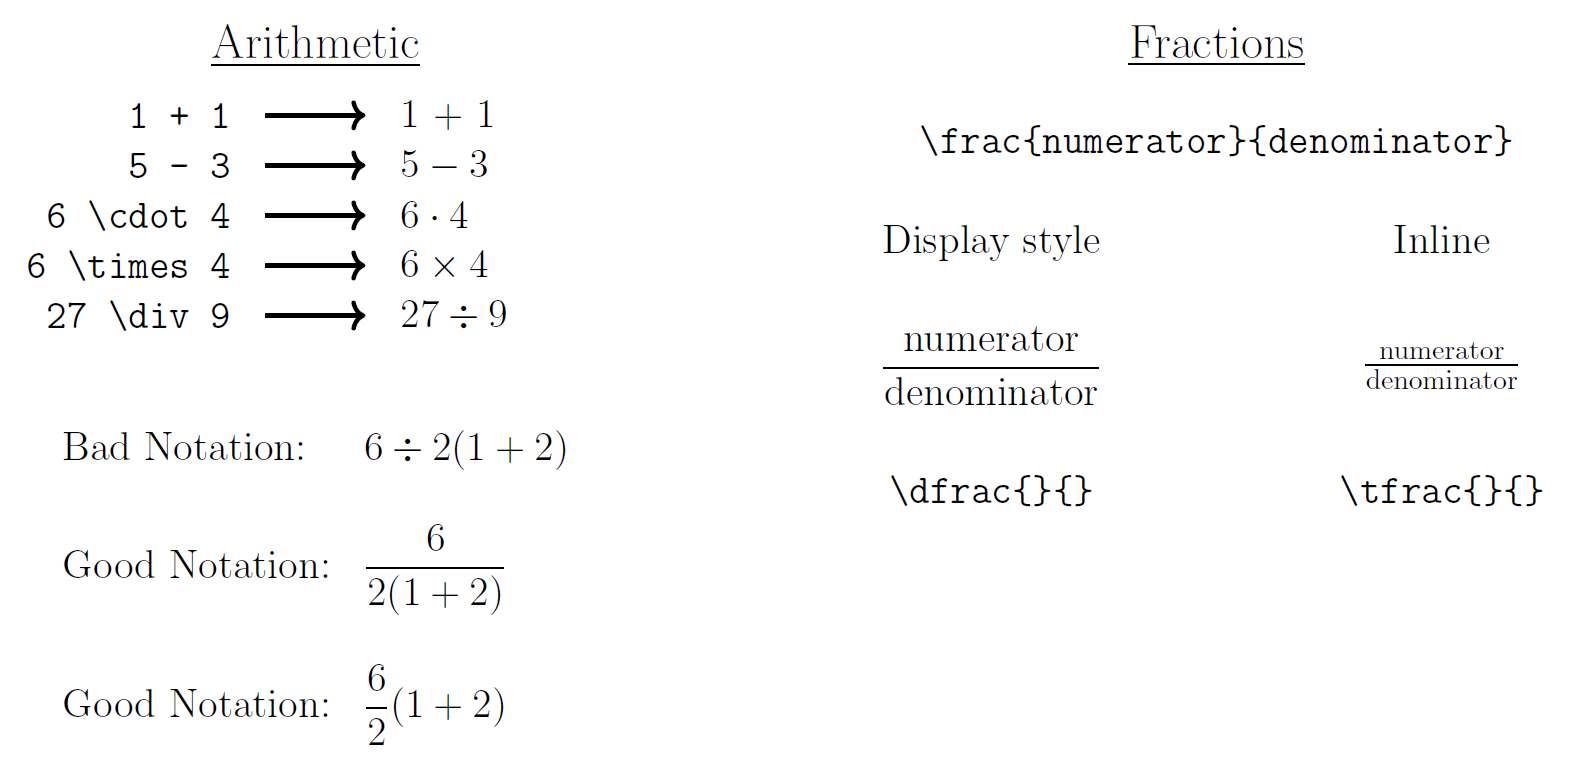
\includegraphics[scale=0.25]{figs/img-3-3.png}
\end{center}
\end{frame}
%=========================================================
\begin{frame}
\begin{center}
    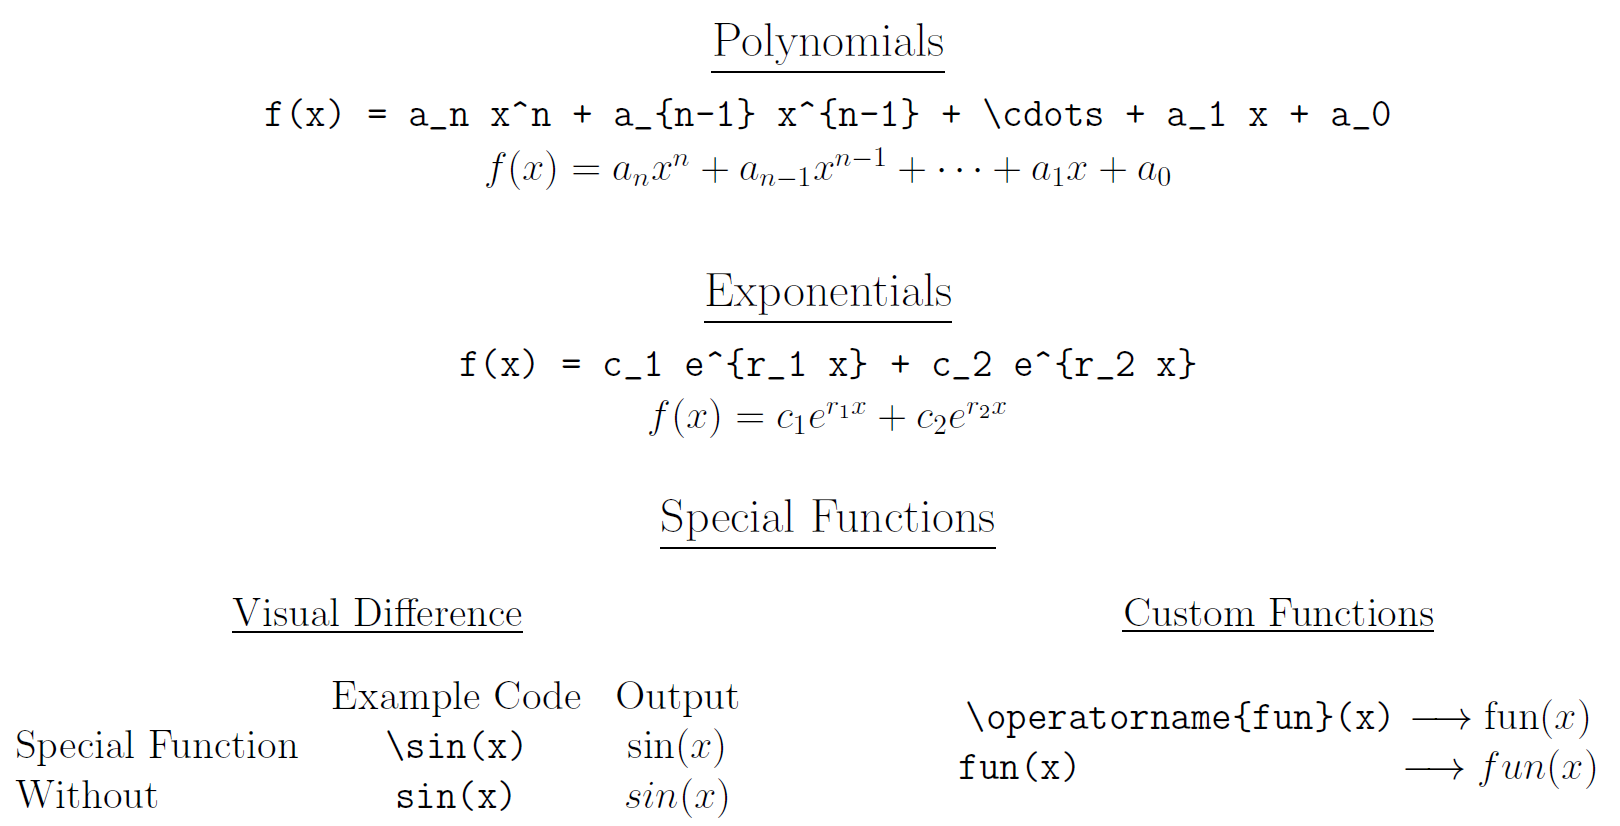
\includegraphics[scale=0.25]{figs/math4.png}
\end{center}
\end{frame}
%=========================================================
\begin{frame}
  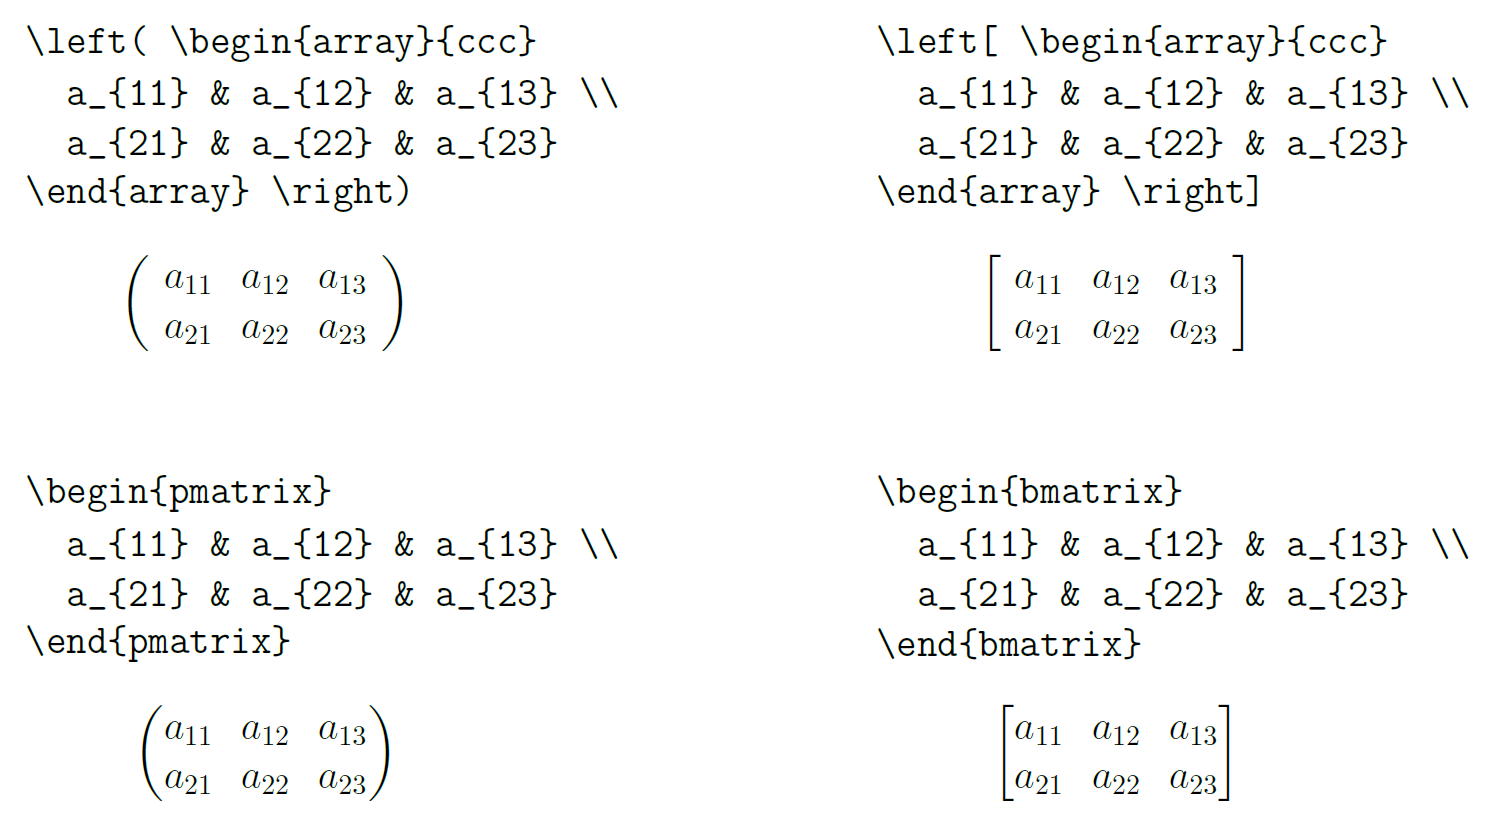
\includegraphics[scale=0.25]{figs/math2.png}
\end{frame}
%=========================================================
\begin{frame}
\begin{center}
  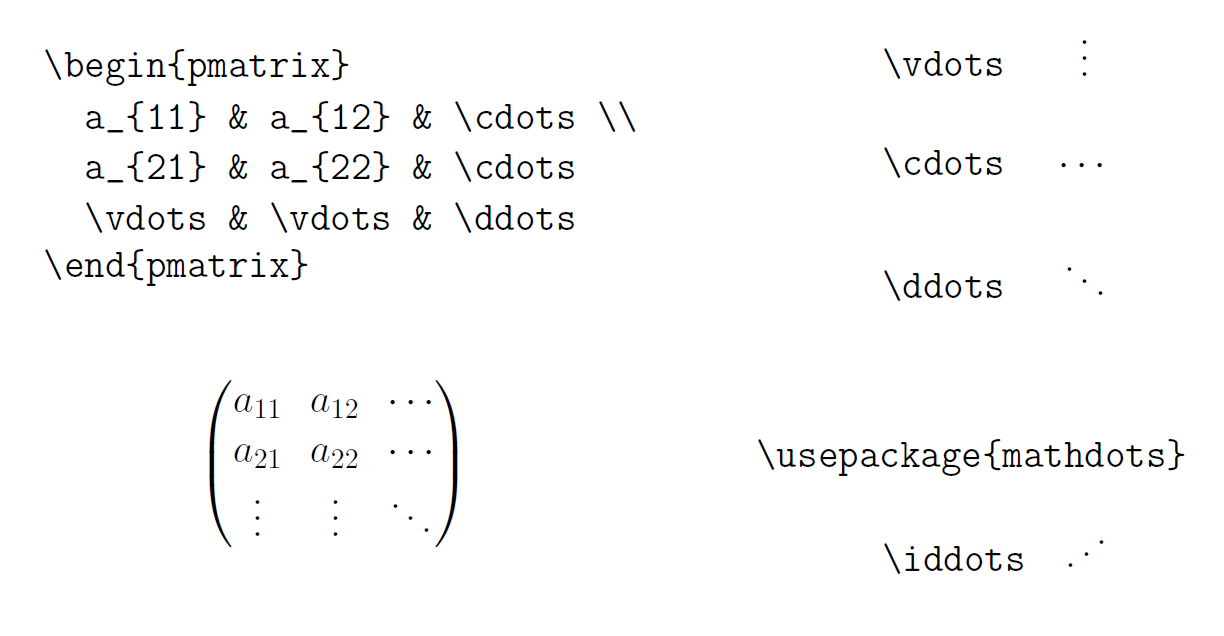
\includegraphics[scale=0.25]{figs/math3.png}
\end{center}
\end{frame}
%=========================================================
\begin{frame}
\begin{center}
  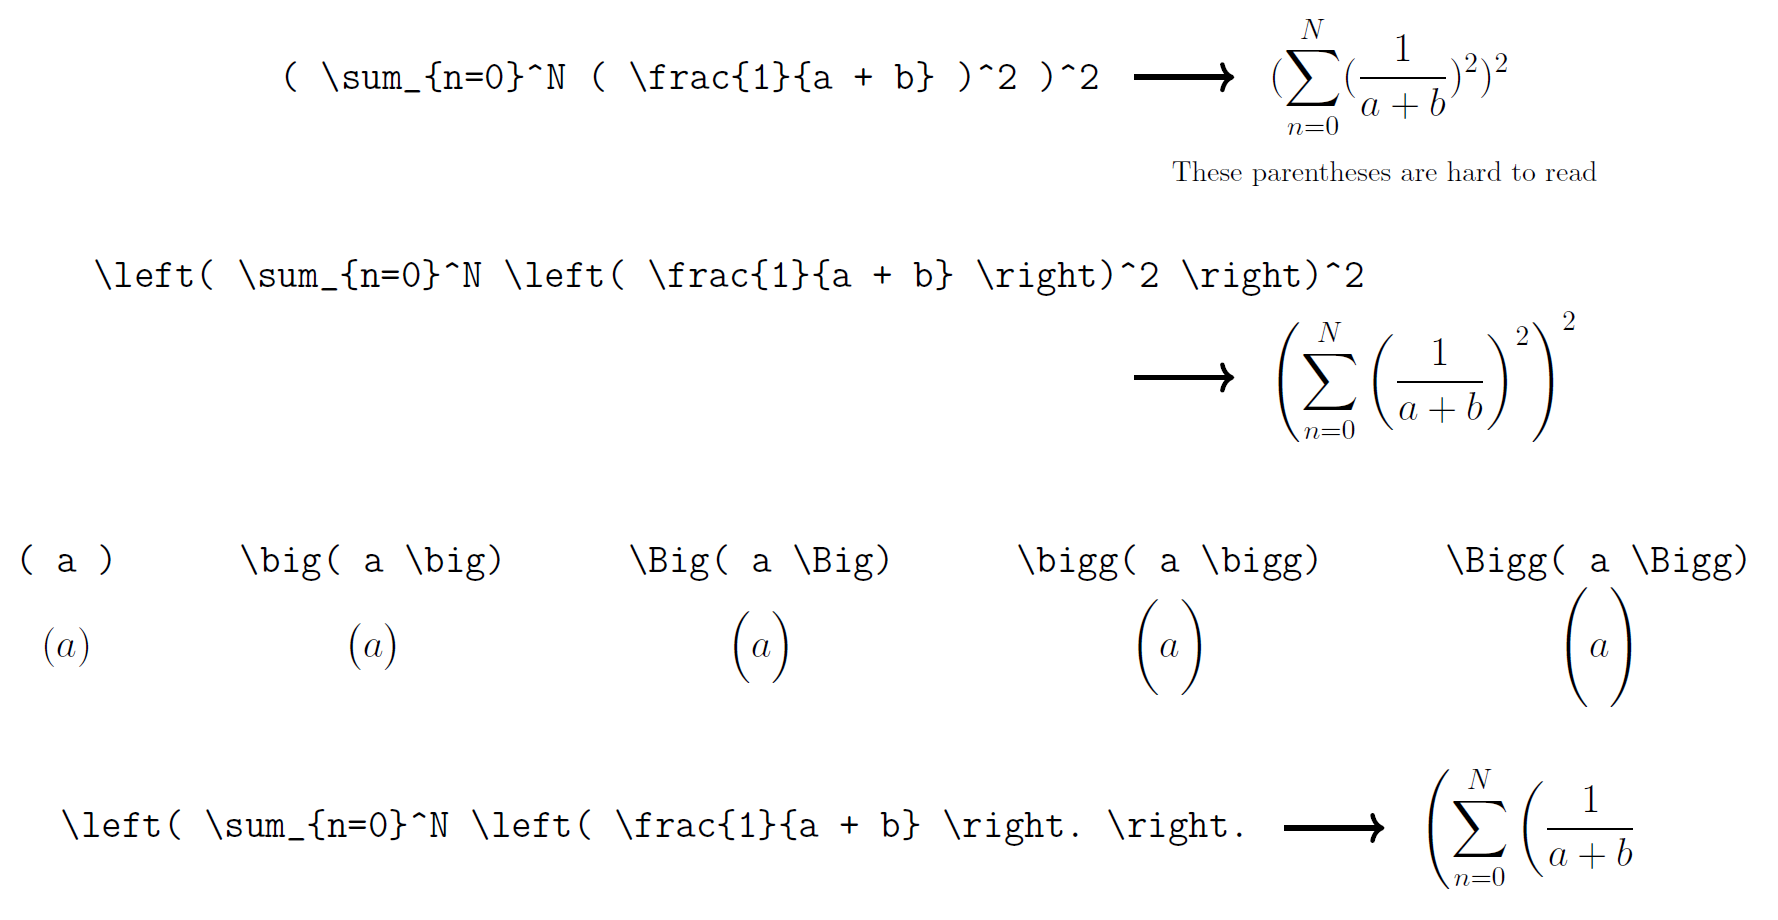
\includegraphics[scale=0.25]{figs/img-3-5.png}
\end{center}
\end{frame}
%=========================================================
\begin{frame}
\begin{center}
  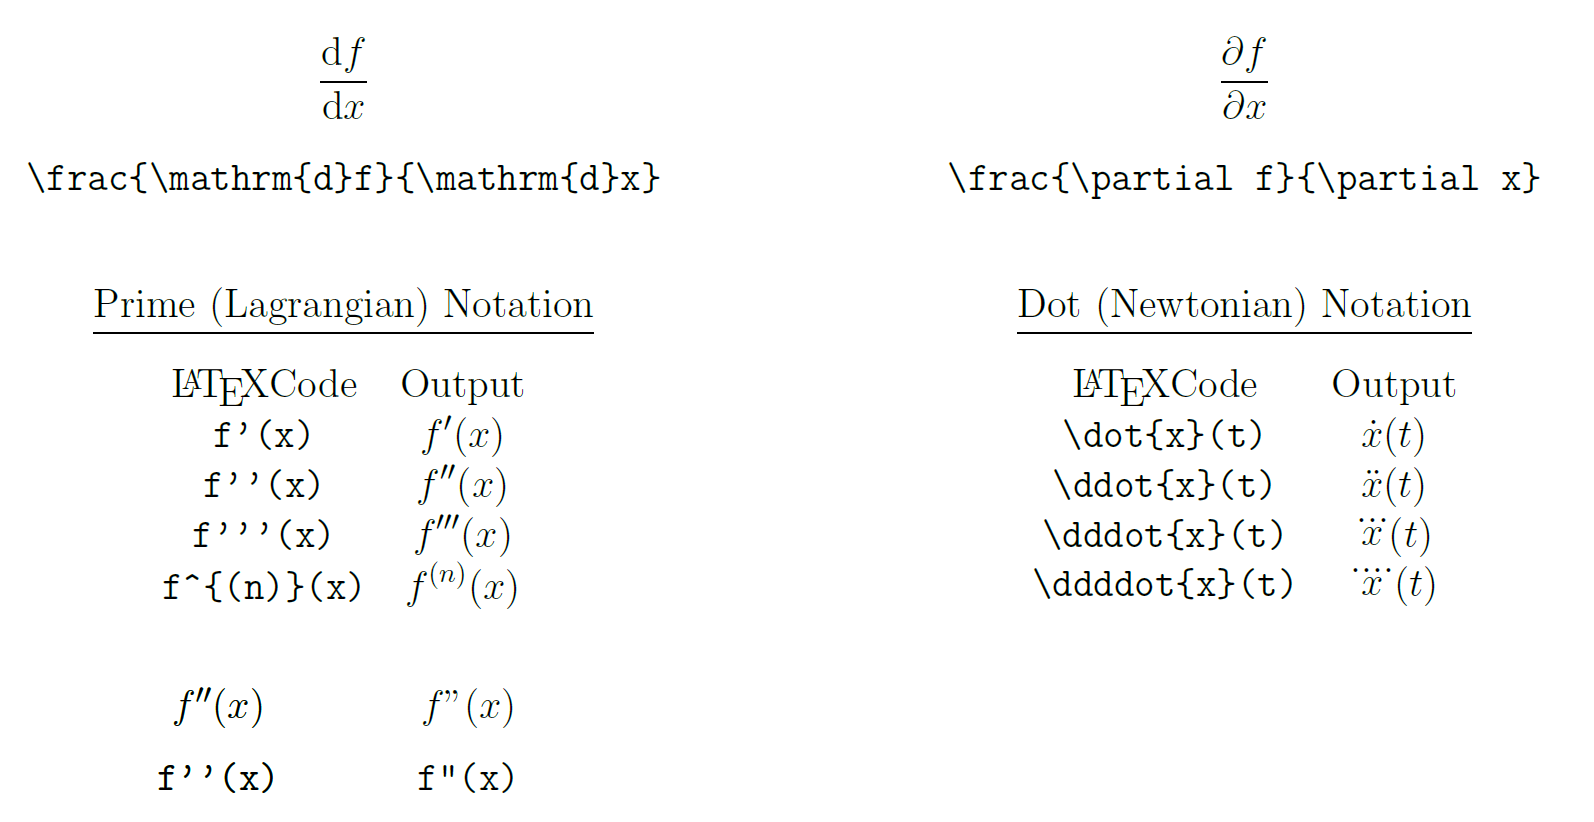
\includegraphics[scale=0.25]{figs/math5.png}
\end{center}
\end{frame}
%=========================================================
\begin{frame}
\begin{center}
  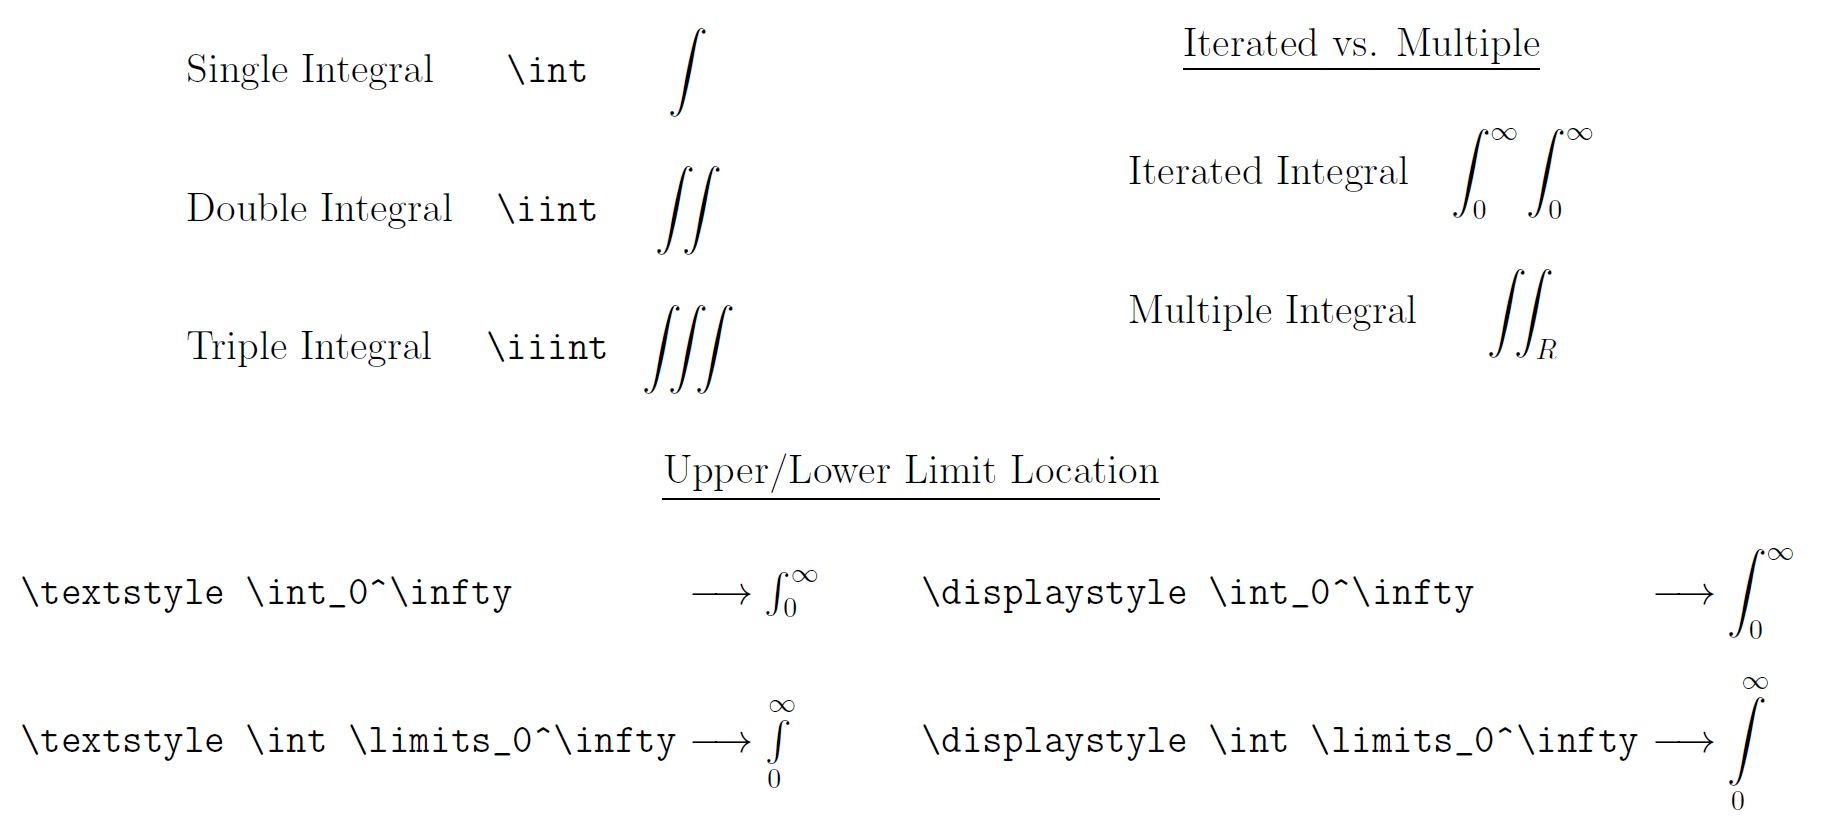
\includegraphics[scale=0.2]{figs/img-5-5.png}
\end{center}
\end{frame}
%=========================================================
\begin{frame}
\begin{center}
  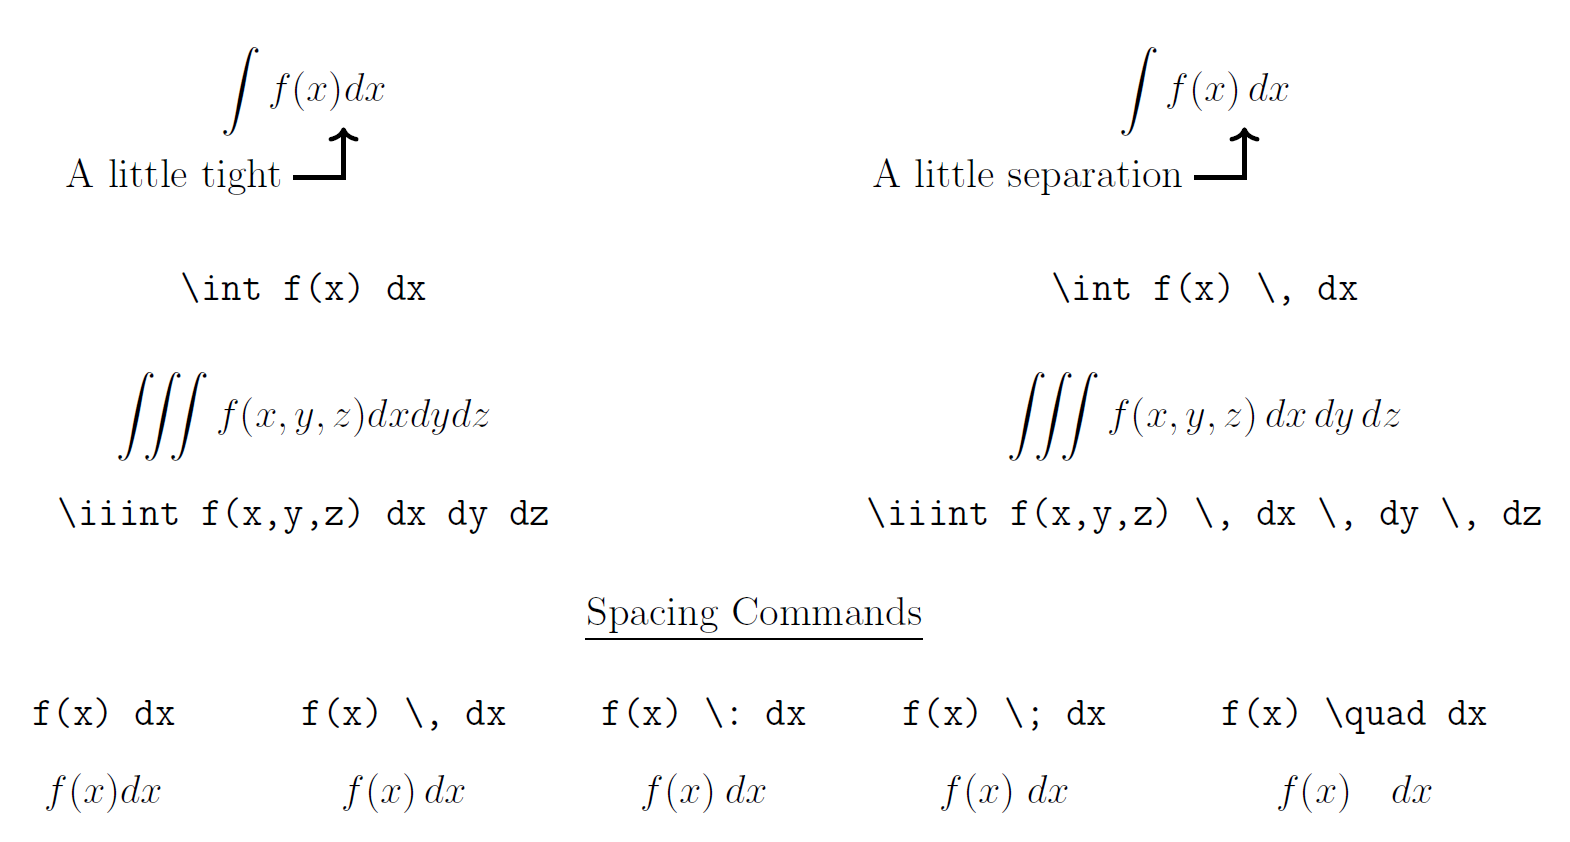
\includegraphics[scale=0.25]{figs/img-5-6.png}
\end{center}
\end{frame}
%=========================================================
\begin{frame}
\begin{center}
  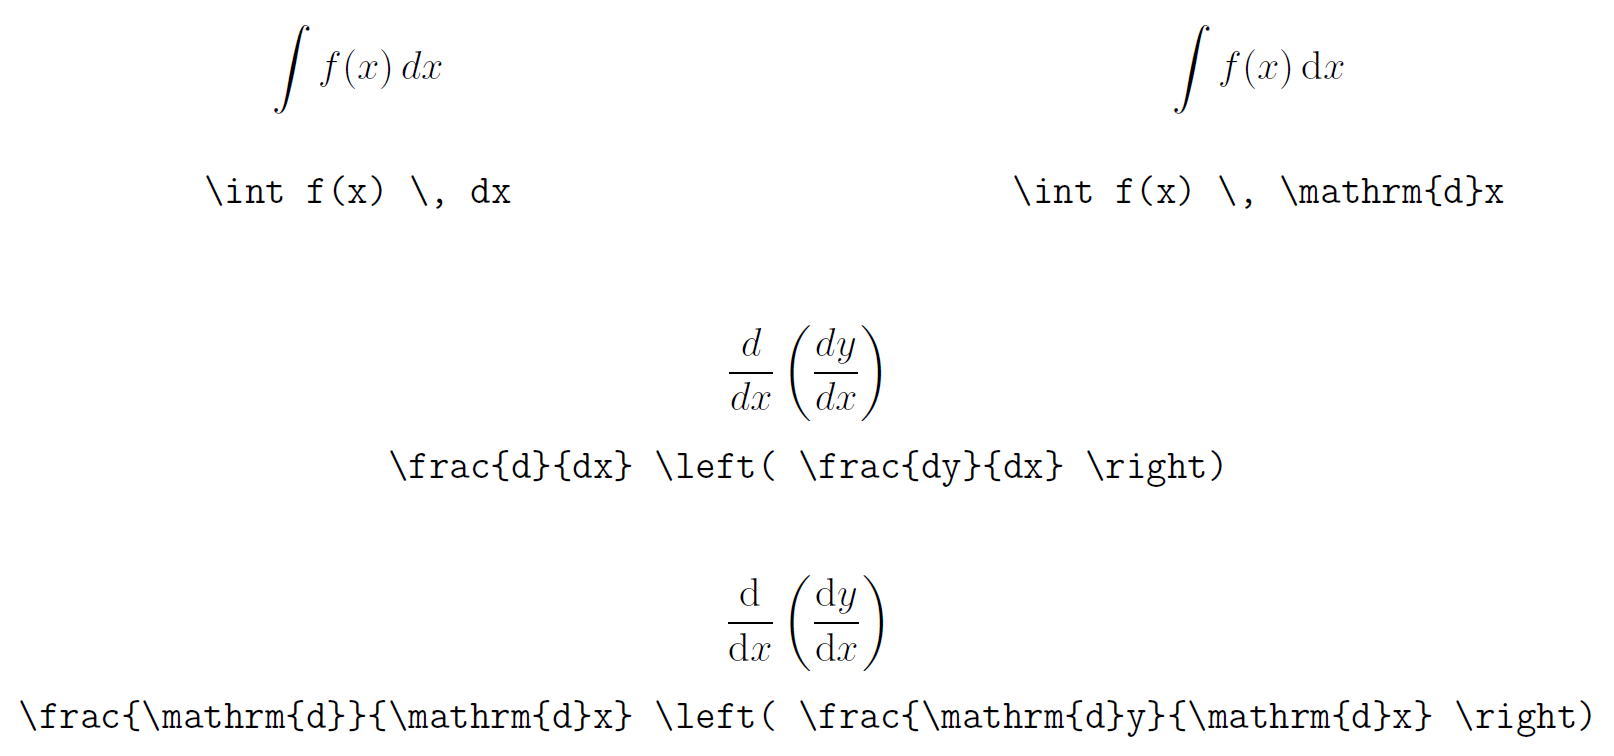
\includegraphics[scale=0.25]{figs/img-5-7.png}
\end{center}
\end{frame}
%=========================================================
\begin{frame}
\begin{center}
    
\includegraphics[scale=0.5]{figs/funny.jpg}
\end{center}
\end{frame}
%=========================================================
\section{إنشاء الببليوجرافيات والاستشهادات}
\scriptsize
\begin{frame}{إنشاء الببليوجرافيات والاستشهادات}
\begin{itemize}\RTListe
    \item :BibTeX هو برنامج لإدارة المراجع لتنسيق قوائم المراجع والاستشهادات النصية في ضمن نظام التنضيد \LaTeX.
\end{itemize}
\begin{center}
    \dbcommand{usepackage}{ biblatex }\\
    \sncommand{addbibresource}\\
    \sncommand{printbibliography}
\end{center}
\begin{itemize}\RTListe
    \item قم بإنشاء ملف بامتداد .bib. على سبيل المثال: MYrefs.bib
    \item استخدم الأمر \dbcommand{ addbibresource }{ MYrefs.bib } لادراج ملف المراجع ضمن ملف العمل
    \item استخدم الأمر \dbcommand{cite}{ Citekey } للاشارة الى اي مرجع ترغب في الاستشهاد به ضمن محتواك النصي
    \item في نهاية ملف العمل استخدم الأمر \sncommand{printbibliography} لضمان ظهور قائمة المراجع، و التى تم الاستشهاد بها ضمن النص.
\end{itemize}
\end{frame}
%=========================================================
\begin{frame}{محتوى الملف ذو الإمتداد bib}
\scriptsize
\begin{center}
    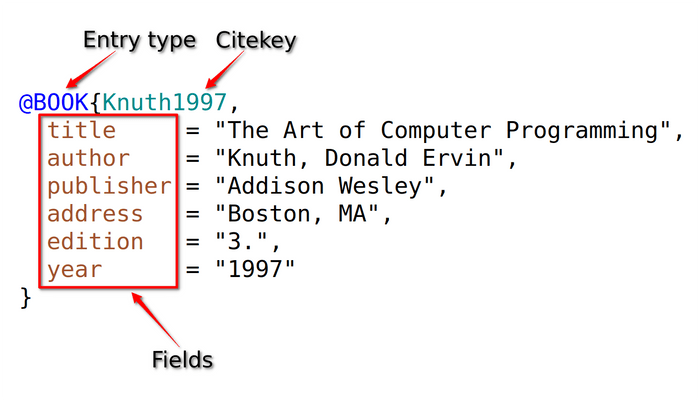
\includegraphics[scale=0.4]{figs/bibtex-format-700x402.png}
\end{center}
\end{frame}
%=========================================================
\begin{frame}{ااستحدام Google Scholar لتجميع الاستشهادات}
\scriptsize
\begin{center}
    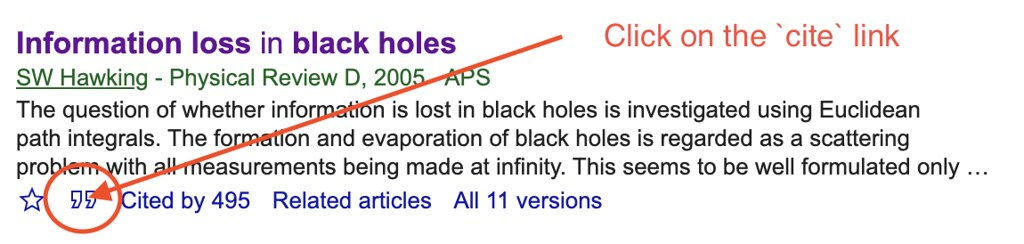
\includegraphics[scale=0.35]{figs/2.jpg}
    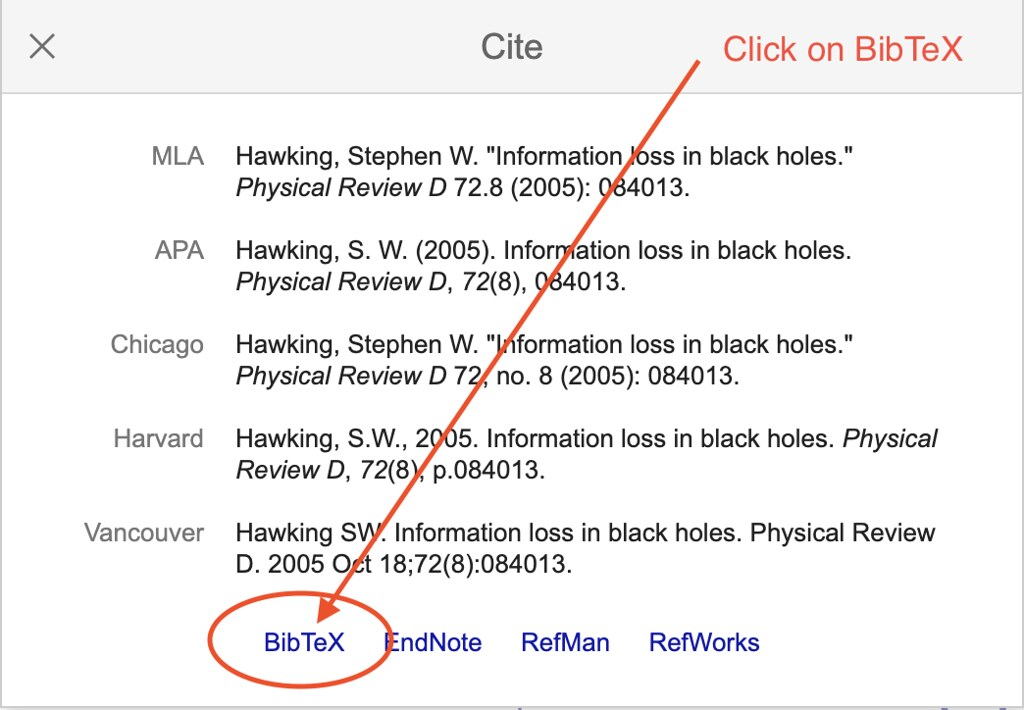
\includegraphics[scale=0.4]{figs/3.jpg}
\end{center}
\end{frame}
%=========================================================
\begin{frame}{استحدام Google Scholar لتجميع الاستشهادات}
\scriptsize
\begin{center}
    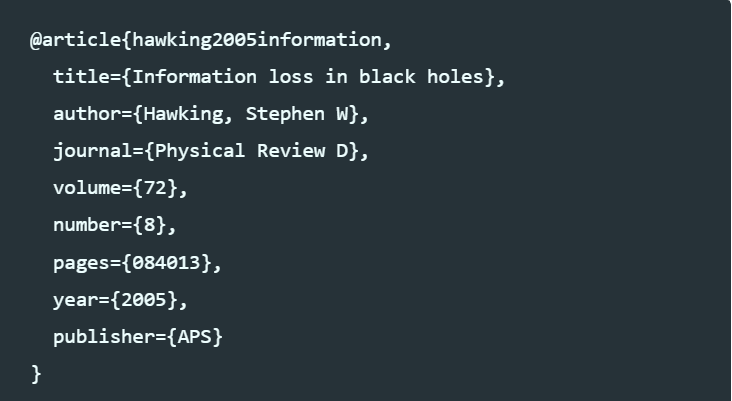
\includegraphics[scale=0.5]{figs/5.png}\\
     \dbcommand{cite}{ hawking2005information }
\end{center}
\end{frame}
%=======================================================
\end{document}